\documentclass[aspectratio=169,
				xcolor=table]{beamer}
				
% Load general definitions
\usepackage[utf8]{inputenc}
%\usepackage[T1]{fontenc}
\usepackage[brazil]{babel}
\usepackage{amsmath}
\usepackage{amsfonts}
\usepackage{amssymb}
\usepackage{graphicx}
\usepackage{verbatim}
\usepackage{cancel}
\usepackage{askmaps}
\usepackage{tabularx}
\usepackage[table]{xcolor}
%\usepackage{tikz}
\usepackage{multirow}
\usepackage{mathtools}
\usepackage{color, colortbl}
\usepackage{etoolbox}
\usepackage{pbox}
\usepackage{changepage}
\usepackage{xpatch}
\usepackage{array}
\usepackage{marvosym}
\usepackage{tabu}
\usepackage{multicol}
\usepackage{listings}
\usepackage{underscore}
\usepackage{filecontents}
\usepackage[]{algorithm2e}
\usepackage{ragged2e}

\newcolumntype{P}[1]{>{\centering\arraybackslash}m{#1}}
\definecolor{Gray}{gray}{0.75}
\definecolor{Gray2}{gray}{0.85}

\definecolor{lightBlue}{HTML}{DAE8FC}
\definecolor{Blue}{RGB}{51, 51, 204}

%\useinnertheme[lily]{rounded}
\usetheme{UniEvangelica}
%\usetheme{Copenhagen}
%\usetheme{Berlin}
%\usecolortheme{dolphin}
\tolerance=1
\emergencystretch=\maxdimen
\hyphenpenalty=10000
\hbadness=10000

\setbeamertemplate{navigation symbols}{}%remove navigation symbols


\let\olditem=\item% 
\renewcommand{\item}{\olditem \justifying}%
\def\center{\trivlist \centering\item\relax}
\def\endcenter{\endtrivlist}

\setbeamertemplate{itemize/enumerate body begin}{\large}
\setbeamertemplate{itemize/enumerate subbody begin}{\large}

\setbeamertemplate{itemize item}{\raisebox{0.1ex}{$\blacktriangleright$}\hskip0.1em}
\setbeamertemplate{itemize subitem}{\raisebox{0.1ex}{$\blacktriangleright$}\hskip0.1em}

\newcommand{\greenarrow}{\textcolor{green}{\rotatebox[origin=c]{180}{\MVArrowDown}}}

\newcommand{\redarrow}{\textcolor{red}{\MVArrowDown}}

%\newcommand{\ftable}{
%	\begin{table}
%		\large
%		\centering
%		\rowcolors{1}{\ifnumless{\rownum}{2}{Blue}{lightBlue}}{}
%}

\newenvironment{eftable}{
	\begin{table}
		\large
		\centering
		\rowcolors{1}{}{Blue}
		\rowcolors{1}{\ifnumless{\rownum}{2}{Blue}{lightBlue}}{}
	}
	{
	\end{table}
}


%\setbeamertemplate{frametitle}
%{
%	%\vspace*{-2em}	
%	\insertframetitle
%
%	 %\textcolor{white}{\LARGE \insertframetitle}
%
%}

% Specific definitions
\institute[]{\uppercase{Engenharia de Software}}
\title[]{Arquitetura e Organização de Computadores}
\subtitle[]{\uppercase{Memória Cache}}
\author[]{Prof. Alexandre Tannus}
\date{}

\AtBeginSection{\frame{\tableofcontents[currentsection]}}

\begin{document}

	\begin{frame}
		\titlepage
	\end{frame}
	
	\begin{frame}{Objetivos}
		\begin{itemize}
			\item Descrever a função das memórias cache 
			\vspace{1em}
			\item Relatar a evolução da memória cache
			\vspace{1em} 
			\item Explicar os princípios de localidade
			\vspace{1em} 
			\item Calcular a eficiência de uma memória cache
			\vspace{1em} 
			\item Distinguir entre as políticas de alocação, substituição e escrita
		\end{itemize}
	\end{frame}

%	\begin{frame}{Metodologia}
%		\begin{itemize}
%			\item O tema da aula é exposto pelo professor em sala de aula. Os alunos interagem durante a apresentação para resolução de dúvidas e exposição de questionamentos relevantes ao tema, os quais podem ser sanados diretamente pelo professor ou serem colocados em discussão pela turma. 
%			\vspace{1em}
%			\item Ao final da exposição do conteúdo são resolvidos exercícios de fixação, para melhor compreensão do tema. As questões podem ser retiradas de concursos públicos, ENADE, POSCOMP ou de autoria do próprio professor.
%		\end{itemize}
%	\end{frame}


	\begin{frame}
		\tableofcontents		
	\end{frame}	
	
	\section{Introdução}

	\begin{frame}
		\frametitle{Memória Cache}
		\begin{itemize}
			\item Memória mais próxima dos registradores
			\begin{itemize}
				\item Acesso mais rápido
				\item Capacidade pequena
			\end{itemize}
		\end{itemize}
		\begin{figure}[hbtp]
			\centering
			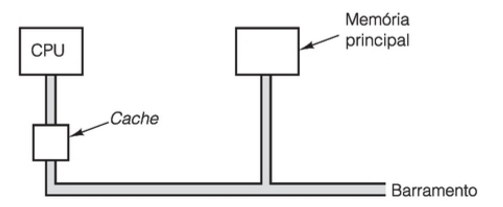
\includegraphics[width=0.7\textwidth, keepaspectratio]{../figs/cap06/cache.png}
		\end{figure}		
	\end{frame}

	\begin{frame}{Memória Cache}

		\begin{figure}[hbtp]
			\centering
			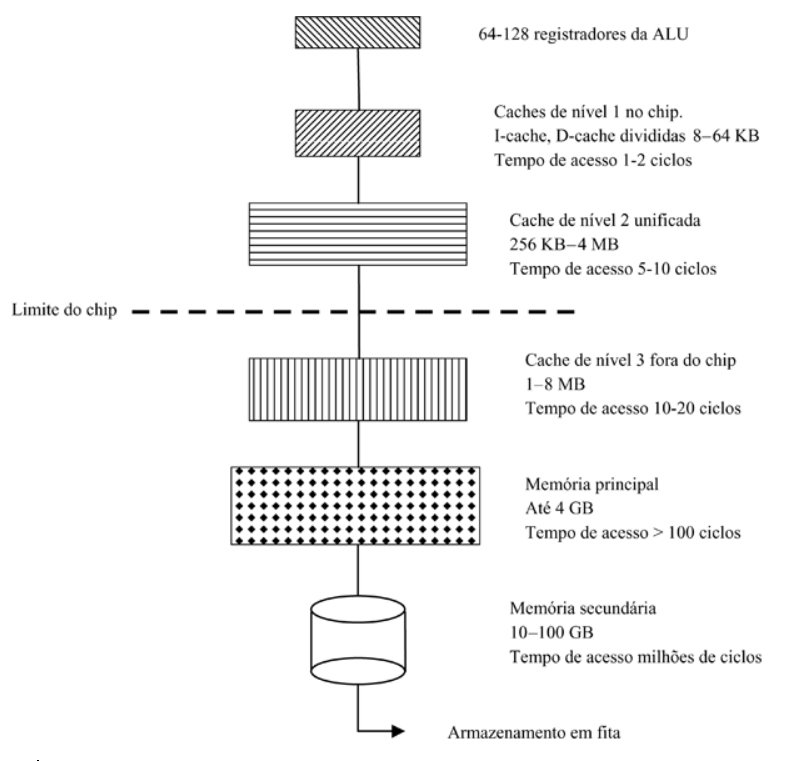
\includegraphics[height=0.8\textheight, keepaspectratio]{../figs/cap07/hierarquia.png}
		\end{figure}		
	\end{frame}
	
	\begin{frame}
		\frametitle{Memória Cache}
		\begin{itemize}
			\item Primeiro local que o processador busca informações (dados ou instruções)
			\vspace{1em}
			\item Pode estar localizada dentro ou fora do processador
			\vspace{1em}
			\item Possibilidade de vários níveis
			\begin{itemize}
				\item Itanium 64 bits: 4 níveis (L1, L2, L3, L4)
			\end{itemize}

		\end{itemize}
	\end{frame}

	\section{Evolução}
	\begin{frame}
		\frametitle{Evolução do cache}
		
		\begin{figure}[hbtp]
			\centering
			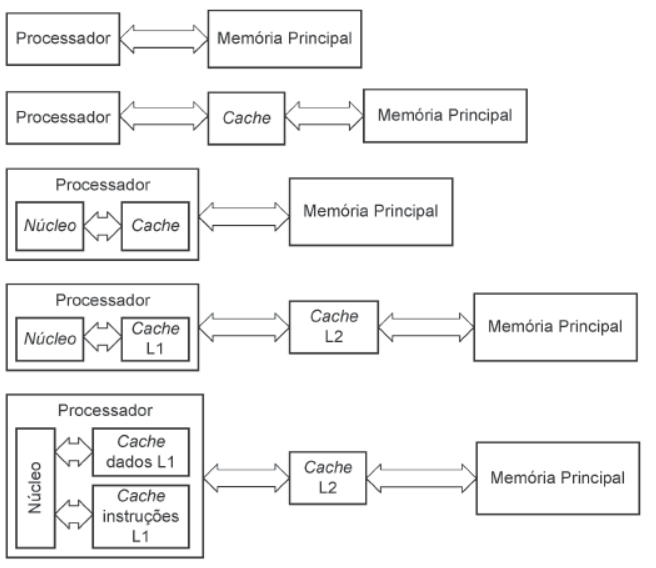
\includegraphics[height=0.8\textheight, keepaspectratio]{../figs/cap06/evolucao1.png}
		\end{figure}
	\end{frame}

	\begin{frame}
		\frametitle{Evolução do cache}
		
		\begin{figure}[hbtp]
			\centering
			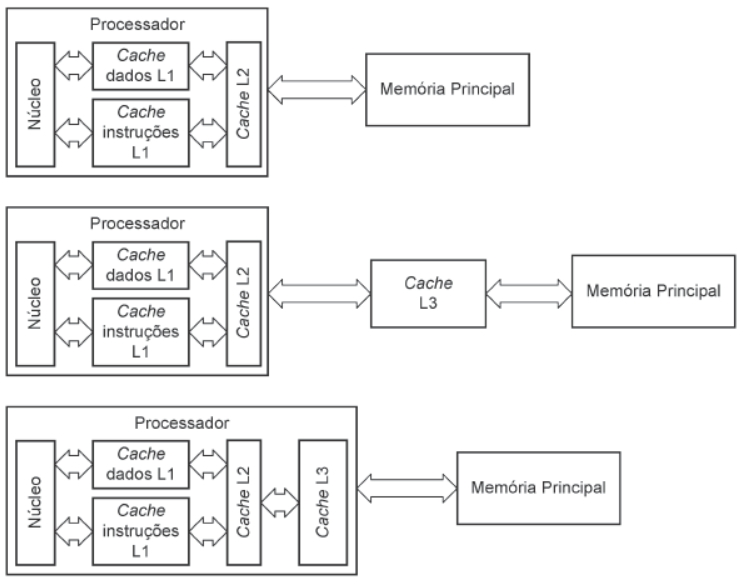
\includegraphics[height=0.8\textheight, keepaspectratio]{../figs/cap06/evolucao2.png}
		\end{figure}
	\end{frame}		
	
	\begin{frame}
		\frametitle{Memórias cache de 1 nível}
		\begin{figure}[hbtp]
			\centering
			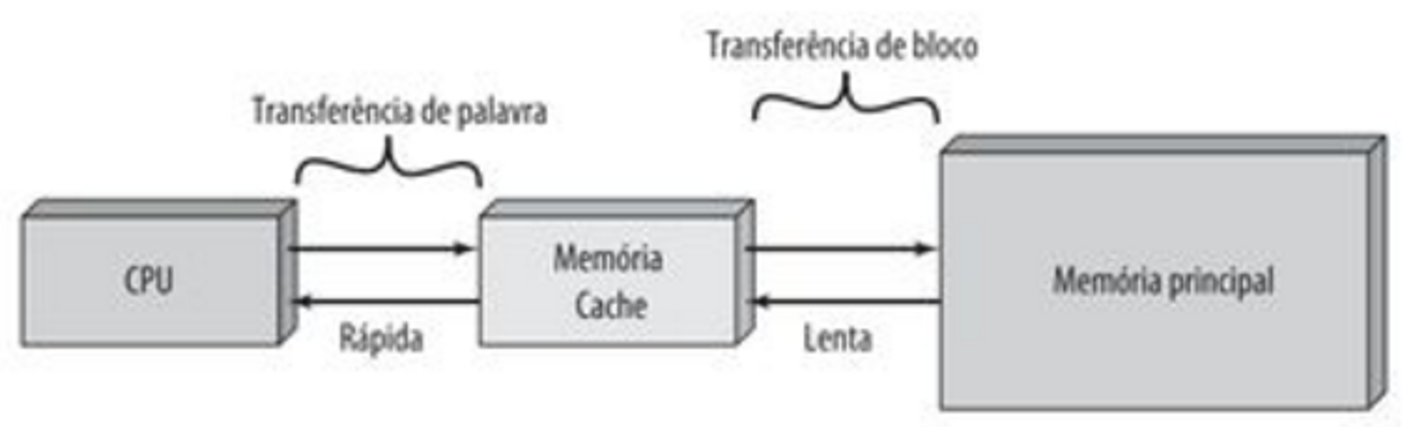
\includegraphics[width=0.9\textwidth, keepaspectratio]{../figs/cap06/cache2.png}
		\end{figure}
	\end{frame}
	
	\begin{frame}
		\frametitle{Memórias cache de vários níveis}
		\begin{figure}[hbtp]
			\centering
			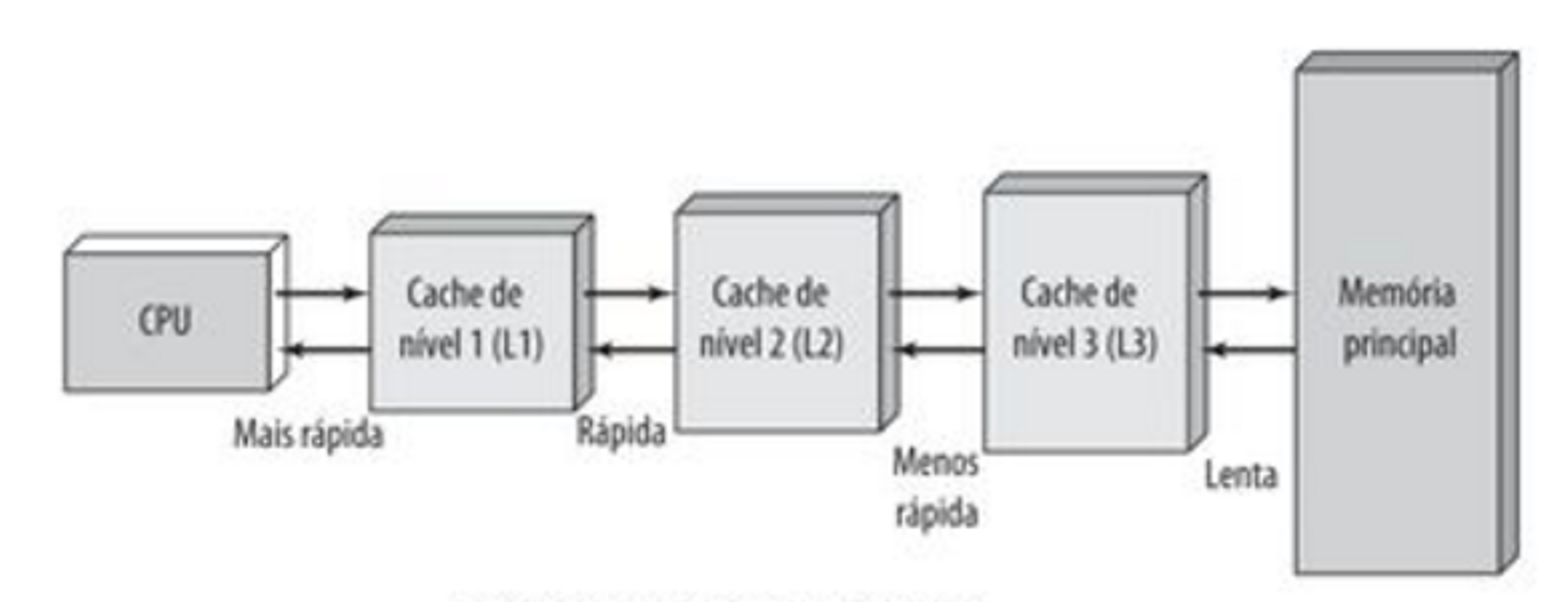
\includegraphics[width=0.9\textwidth, keepaspectratio]{../figs/cap06/cache3.png}
		\end{figure}
	\end{frame}

	\section{Funcionamento}

	\begin{frame}{Funcionamento}
		\begin{figure}[hbtp]
			\centering
			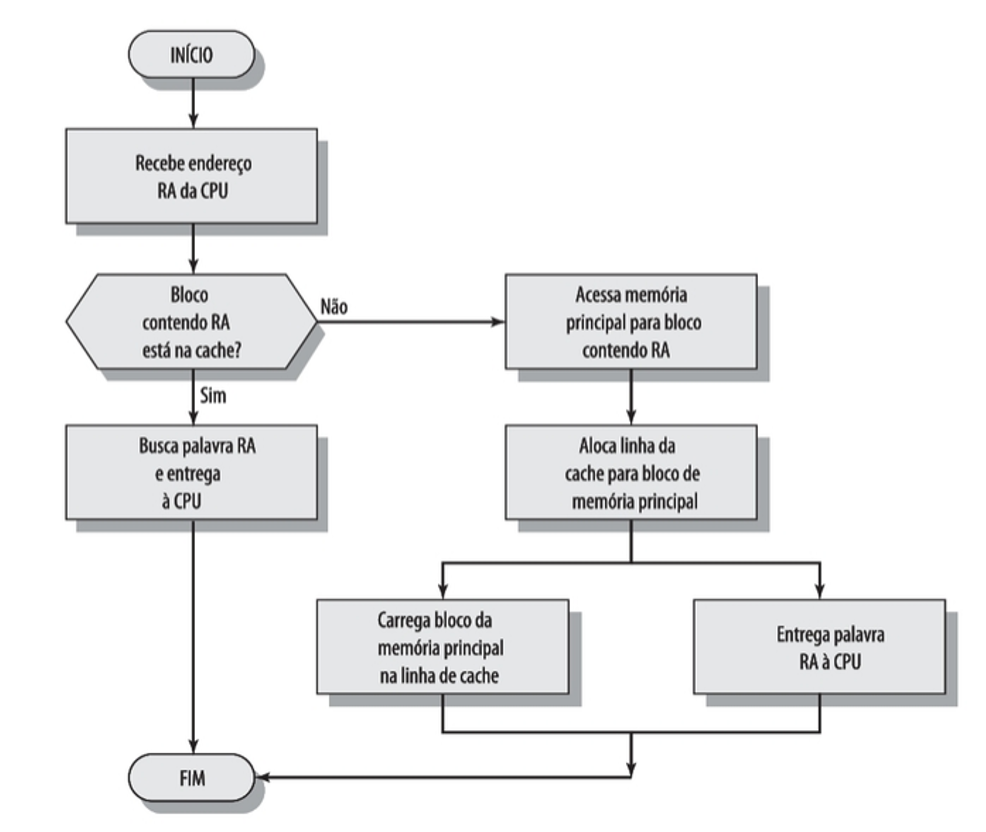
\includegraphics[height=0.8\textheight, keepaspectratio]{../figs/cap06/cacheFunc.png}
		\end{figure}
	\end{frame}

%	\begin{frame}{Questão - BRDE 2012}
%		\begin{enumerate}[I]
%			\item A ideia básica de uma memória Cache simples é: as palavras de memórias usadas com maior frequência são mantidas na cache. 
%			\item A localização lógica da cache é entre a CPU e a memória principal. 
%			\item Usando o princípio da localidade como guia, memórias principais e cache são divididas em blocos de tamanhos variáveis. 
%			\item O projeto de cache é uma questão de importância cada vez maior para CPUs de alto desempenho. Embora quanto maior a cachê, maior o custo. 
%		
%		\end{enumerate}
%
%
%	\end{frame}


	\begin{frame}{Princípio da localidade}
		\begin{itemize}
			\item Localidade espacial
			\begin{itemize}
				\item Quando um determinado item é referenciado, itens com endereços de memória próximo a ele tendem a ser logo referenciados
			\end{itemize}
			\vspace{1em}
			\item Localidade temporal
			\begin{itemize}
				\item Quando um determinado item é referenciado, a tendência é que ele seja novamente referenciado dentro de um curto período de tempo
			\end{itemize}
		\end{itemize}
	\end{frame}

	\begin{frame}{Parâmetros importantes}
		\begin{itemize}
			\item Tamanho da cache
			\item Tamanho dos blocos
			\item Taxa de sucesso (\textit{hit ratio}) / insucesso (\textit{miss ratio})
			\item Política de alocação
			\item Política de substituição
			\item Política de escrita
		\end{itemize}
	\end{frame}
	
	\begin{frame}{Blocos de memória}
		\begin{itemize}
			\item A memória cache é organizada em blocos (linhas de cache)
			\vspace{1em}
			\item Armazena cópias de parte da memória principal
			\vspace{1em}
			\item Contém um identificador (\textit{tag}) da posição da memória principal onde se encontram os dados
		\end{itemize}
	\end{frame}	

	\begin{frame}{Blocos de Memória}

		\begin{figure}[hbtp]
			\centering
			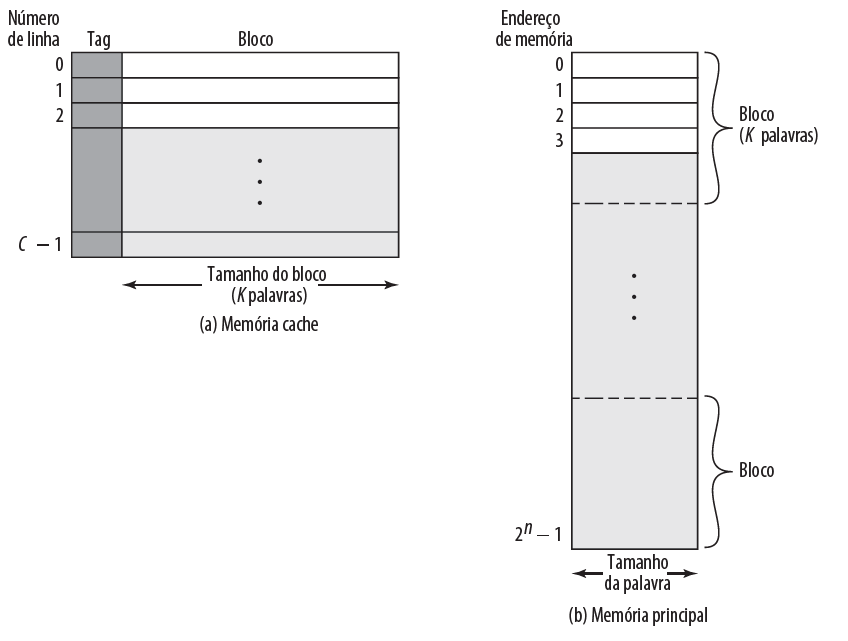
\includegraphics[height=6.5cm, keepaspectratio]{../figs/cap06/blocosCache.png}
		\end{figure}		
	\end{frame}
	
	\begin{frame}{Taxa de sucesso/insucesso}

		\begin{itemize}
			\item Taxa de sucesso (\textit{hit ratio})
			\begin{itemize}
				\item Percentual de vezes que a palavra buscada está presente na cache
				\item Ideal: acima de 95%
			\end{itemize}			
			\vspace{1em}
			\item Taxa de insucesso (\textit{miss ratio})
			\begin{itemize}
				\item Percentual de vezes que a palavra buscada está ausente na cache				
			\end{itemize}
		\end{itemize}	
	
	\end{frame}
	
	\begin{frame}
		\frametitle{Política de Alocação}
		\begin{itemize}
			\item Determina o local de armazenamento de uma linha de dados
			\vspace{1em}
			\item Políticas mais flexíveis geram maior custo de hardware
		\end{itemize}
	\end{frame}
	
	\begin{frame}{Mapeamento Direto}
		\begin{itemize}
			\item Forma mais simples de localização do bloco
			\item Utiliza os $P$ bits menos significativos do número do bloco como índice
			\item Cada bloco da memória principal mapeia uma linha exclusiva de cache
			\item Vantagem
			\begin{itemize}
				\item Simplicidade de implementação
			\end{itemize}
			\item Desvantagem
			\begin{itemize}
				\item \textit{Thrashing} - Baixa taxa de sucesso e contínua troca de blocos na cache
			\end{itemize}
		\end{itemize}
	\end{frame}	
	
	\begin{frame}
		\frametitle{Mapeamento Direto}
		\begin{figure}[hbtp]
			\centering
			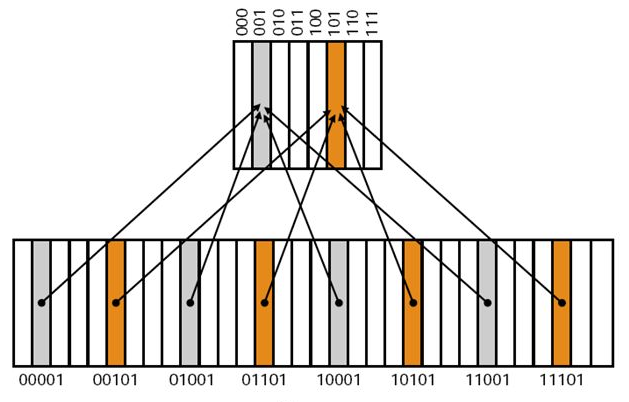
\includegraphics[height=0.8\textheight, keepaspectratio]{../figs/cap06/cachedireto.png}
		\end{figure}		
	\end{frame}
	
	\begin{frame}{Mapeamento Associativo}
		\begin{itemize}
			\item Permite o carregamento de um bloco em qualquer linha de cache
			\item Linhas são substituídas somente em caso de memória cheia
			\item Vantagem
			\begin{itemize}
				\item Melhor utilização da cache
				\item Maior taxa de acertos
			\end{itemize}
			\item Desvantagem
			\begin{itemize}
				\item Circuitos de controle mais complexos
				\item Diminuição da capacidade de armazenamento
			\end{itemize}
		\end{itemize}
	\end{frame}

	\begin{frame}{Mapeamento associativo}
		\begin{figure}[hbtp]
			\centering
			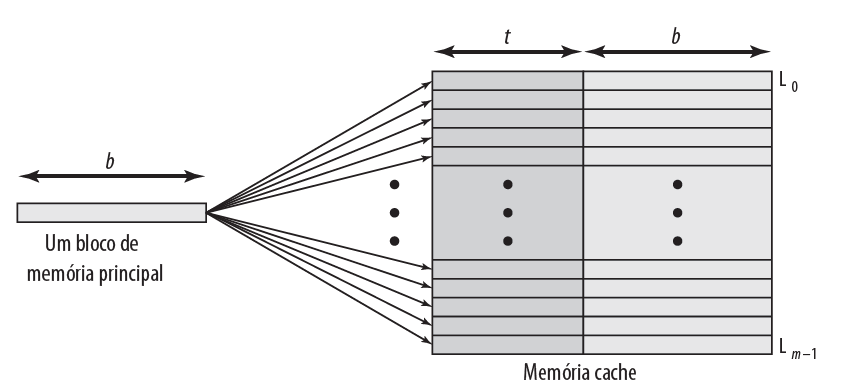
\includegraphics[height=0.8\textheight, keepaspectratio]{../figs/cap06/associativo.png}
		\end{figure}		
	\end{frame}	
	

	\begin{frame}
		\frametitle{Política de substituição}
		\begin{itemize}
			\item Determina qual bloco será sobrescrito caso a cache esteja cheia
			\begin{itemize}
				\item \textit{First In First Out} - FIFO
				\begin{itemize}
					\item O bloco mais antigo na cache será substituído pelo novo
				\end{itemize}
				\item \textit{Least Recently Used} - LRU
				\begin{itemize}
					\item O bloco menos utilizado recentemente é substituído
				\end{itemize}
				\item \textit{Least Frequently Used} - LFU
				\begin{itemize}
					\item O bloco menos frequentemente utilizado é substituído
				\end{itemize}				
				\item Escolha Aleatória
				
			\end{itemize}
		\end{itemize}
	\end{frame}

	\begin{frame}{Políticas de Escrita}
		\begin{itemize}
			\item Escrita imediata (\textit{write-through})
			\item Escrita atrasada (\textit{write-back})
		\end{itemize}
	\end{frame}

	\begin{frame}{Escrita imediata (write-through)}
		\begin{itemize}
			\item Memória principal e cache são atualizadas simultaneamente.
			\vspace{1em}		 
			\item Vantagem
			\begin{itemize}
				\item Consistência da cache em relação à memória principal
			\end{itemize}
			\vspace{1em}
			\item Desvantagem
			\begin{itemize}
				\item Pode causar alto tráfego de memória				
			\end{itemize}		
		
		\end{itemize}
		
	\end{frame}
	
	\begin{frame}{Escrita atrasada (write-back)}
		\begin{itemize}
			\item Escrita apenas na memória cache
			\vspace{1em}
			\item Memória principal é atualizada quando a linha é substituída
			\vspace{1em}
			\item Vantagem
			\begin{itemize}
				\item Consistência da cache em relação à memória principal
			\end{itemize}
			\vspace{1em}
			\item Desvantagem
			\begin{itemize}
				\item Pode causar alto tráfego de memória				
			\end{itemize}			
		\end{itemize}
	\end{frame}
	
%	\begin{frame}{Falhas em memórias cache}
%		\begin{itemize}
%			\item Falhas compulsórias
%			\item Falhas de conflito
%			\item Falhas de capacidade
%		\end{itemize}
%	\end{frame}	

	\begin{frame}{Coerência de cache}
		\begin{itemize}
			\item \alert{Problema:} Memórias compartilhadas podem apresentar inconsistência nos dados
			\vspace{1em}
			\item Soluções para o problema (coerência)
			\begin{itemize}
				\item Observação do barramento com \textit{write-through}
				\item Transparência de hardware
				\item Memória não cacheável
			\end{itemize}
		\end{itemize}
	\end{frame}
	
	\begin{frame}
		\frametitle{Questão - TJ-RJ 2012}
		As designações L1 e L2 são utilizadas em referência à memória de computadores. A seu respeito é correto afirmar que 
		\begin{enumerate}[a]
			\large
			\item memória L1 tem menor latência que memória L2.
			\item memória L1 tem maior latência que memória L2.
			\item todo computador tem ambos os tipos de memória.
			\item nenhum computador pode ter ambos os tipos de memória.
			\item L1 e L2 designam níveis de memória virtual.
		\end{enumerate}
	\end{frame}

	\begin{frame}{Questão - TRT - 4ª REGIÃO (RS) - 2011 }
	Se a referência à memória é para um endereço determinado, é possível que a próxima referência à memória seja feita nas adjacências desse endereço. Trata-se de uma afirmação relevante ao princípio que forma a base de todos os sistemas cache, denominado princípio da 

	\begin{enumerate}[a]
		\item referência.
		\item localidade.
		\item temporalidade.
		\item latência.
		\item velocidade.	
	\end{enumerate}

	
	
	\end{frame}
	
	\begin{frame}
		\frametitle{Questão - Petrobras 2012}
		Qual característica NÃO se refere à memória cache de processadores?
		
		\begin{enumerate}[a]
			\large
			\item Tem o objetivo de reduzir o tempo de acesso à memória principal.
			\item Os dados nela armazenados são cópias de parte da memória principal.
			\item É implementada pelo sistema operacional com suporte do hardware.
			\item Pode ser inserida diretamente no chip do processador.
			\item É comumente encontrada em processadores RISC.
		\end{enumerate}
	\end{frame}


	\begin{frame}{Questão - Colégio Pedro II 2016}
		\begin{enumerate}[I]
			\item O número de blocos da memória principal é igual ao número de linhas da memória cache.
			\item No mapeamento direto, é possível que dois acessos recentes façam referência a blocos alocados para mesma linha da memória cache, o que provoca a retirada de um bloco que acabou de ser trazido da memória principal.
			\item Na estratégia de mapeamento associativo, o bloco trazido da memória principal pode ser alocado em qualquer linha da memória cache, de acordo com uma política de substituição de linhas definida.
			\item Denomina-se hit quando um dado solicitado não está armazenado na memória cache e, neste caso, o bloco da memória principal que contém o byte desejado é transferido para a memória cache.
			\item A eficiência da memória cache de um sistema de computação em que ocorrem 94 hits a cada 100 acessos é de 6%.
		\end{enumerate}
			
	
		\end{frame}	


		\begin{frame}{Questão - EBSERH 2016}
		
		Constantemente em material técnico de hardware encontra-se o termo técnico cache. Assinale, das alternativas abaixo, a única que identifica corretamente uma breve descrição de cache: 
		
		\begin{enumerate}[a]
			\item uma área de armazenamento temporária onde os dados frequentemente utilizados são armazenados para acesso rápido.
			\item 	para garantir a qualidade dos dados que circulam entre memórias e processador, o cache armazena temporariamente os dados, processa algoritmos de segurança e somente repassa dados seguros para o próximo dispositivo. 
			\item uma memória de grande capacidade de armazenamento, de alta velocidade e custo bastante baixo.
			\item uma área de armazenamento semelhante a ROM onde os dados são frequentemente acedidos por meio de estatísticas dos dados mais acessados.
			\item uma memória de pequena capacidade de armazenamento, de baixa velocidade e custo bastante alto.		
		\end{enumerate}

	
		\end{frame}

	\begin{frame}{Questão - Petrobras 2012}
		A técnica de atualização da memória cache, na qual as escritas são feitas apenas nessa memória, e a memória principal só é atualizada se o bit de atualização do bloco substituído tiver o valor 1, é denominada
		
		\begin{enumerate}[a]
			\item write-through
			\item write-back
			\item write-on-update
			\item write-if-updated
			\item write-when-updated		
		\end{enumerate}



	\end{frame}	
	\begin{frame}{Bibliografia}
		\nocite{Englander2011}
		\nocite{Paixao2014}
		\nocite{Stallings2010}
    	\bibliographystyle{plain}
    	\bibliography{../refs}   	
	
	\end{frame}		
	
	\begin{frame}{}
	\end{frame}

\end{document}